\label{referencial}

Neste Capítulo apresentamos ...

\section{Engenharia de Software}
 A partir do início da década de 1940, os computadores eram criados com um fim específico, rodando apenas para o fim específico ao qual foi projetado, como por exemplo o Colossus, primeira máquina computacional criada  por Alan Turing que se tem registrado, com o fim de decifrar mensagens criptografadas enviadas pelos alemães\cite{colossus}.
 Engenharia de software é o processo que foca nas áreas de planejamento, desenvolvimento e entrega dos sistemas de software. É com este tipo de metodologia que conseguimos estimar de maneira mais apurada formas de como desenvolver o sistema, estimar prazos, recursos e até mesmo espaços para melhora durante e após a conclusão do projeto. A engenharia de software nasceu da necessidade de entregar ao cliente uma maior garantia de qualidade, sem deixar de lado a preocupação com prazos, estes cada vez mais curtos perante as demandas que o mundo e sua evolução tecnológica tem exigido \cite{Sommerville07}. 

\subsection{Engenharia de Requisitos}
A engenharia de requisitos (ou especificação de software) é a área responsável por entender e decidir quais serão as requisições necessárias ao sistema solictado e verificar os impedimentos relacionados ao desenvolvimento e operação do sistema. Costuma ser um estágio crítico do processo de criação de um software, pois uma vez mal desenhado e com erros nesta fase, mais a frente no projeto, implantação e manutenção do sistema problemas serão comuns de aparecerem \cite{Sommerville07}.

Esta etapa existe com o propósito de criar uma documentação de requisitos acordados onde cria a especificação de um sistema que possa atender às necessidades dos clientes atendidos para o desenvolvimento do software. Usualmente, os requisitos são postos para seus clientes e usuários finais em um nível mais alto, sem grandes detalhes técnicos, enquanto para os desenvolvedores é essencial que os detalhes técnicos sejam muito bem apresentados \cite{Sommerville07}.

De acordo Sommerville \cite{Sommerville07}, são quatro níveis principais do processo de engenharia de requisitos, que são os seguintes:
\begin{enumerate}
    \item \textit{Estudo de viabilidade}: Realiza-se uma aproximação a respeito a possibilidade de se cumprir com as requisições do usuário em questão, valendo-se de tecnologias contemporâneas, seja a nível de software ou de hardware. Esse estudo leva em conta se o sistema a ser criado será lucrativo sobre uma posição de negócio e se o mesmo pode ser construído sob condições financeiras limitadas. Um estudo de viabilidade deve ser algo sem grandes custos e de rápida conclusão, onde o resultado culmina na decisão ou não de continuar com a possibilidade de um estudo mais detalhado.
    \item \textit{Elicitação e análise de requisitos}: Esta é a parte do processo onde se inicia a formação mais aprofundada dos requisitos do sistema por meio da análise de outros sistemas existentes, além de debates com os potenciais clientes/usuários e compradores, verificação de tarefas e outras etapas. É nesta parte onde a criação de protótipos ou modelos de sistemas são feitos para ajudar a elucidar o sistema a ser criado.
    \item \textit{Especificação de requisitos}: A etapa de ação de tradução dos dados e informações coletados durante a etapa de análise de uma documentação que detalha o connjunto de requisitos. Geralmente, são dois os tipos de requisitos que podem ser inseridos nesta documentação. A parte onde o cliente fala o que deseja criar para o seu produto de forma mais geral e sem a profundidade técnica, mais voltada para o objeto de desejo de uso é chamada de requisitos de usuário, enquanto a parte onde há um maior detalhamento na descrição técnica a ser fornecido ao usuário é chamado de requisitos de sistema.
    \item \textit{Validação de requisitos}: Esta etapa é onde verificamos se o sistema está consistente, completo e de acordo com a realidade, onde não por acaso se descobrem os principais erros e a documentação deve ser alterada de forma a visar a correção destes problemas que foram mapeados durante esta etapa.
\end{enumerate}

\begin{figure}
    \centering
    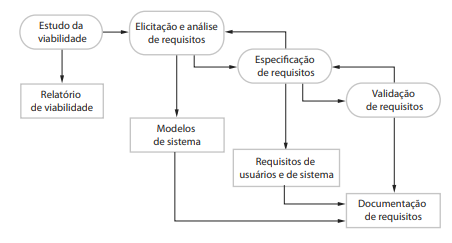
\includegraphics{img/eng_req.png}
    \caption{Gráfico do processo de engenharia de requisitos} \cite{Sommerville07}
    \label{fig:eng_req}
\end{figure}

 Obviamente, para Sommerville \cite{Sommerville07}, de acordo com as atividades decorrentes do processo, tais atividades não são realizadas de forma linear e sequencial. Até alcançar a fase de entrega final, várias iterações novas são pensadas para novas definições, especificações e revisões dos requisitos, mostrando que tais etapas são de certa forma ligadas em cadeia. Nos modelos ágeis de desenvolvimento, como o \textit{extreme programming}, os requisitos são criados, desenvolvidos e entregues de forma a incrementar sempre a iteração anterior de acordo as necessidades básicas e essenciais do usuário, enquanto o processo de elicitação de requisitos é feita pelos usuários que estão testando a ferramenta juntamente com o time de desenvolvedores.
 
 De acordo Fleming \cite{cmmi}, a área de engenharia de requisitos tem em mente três pontos em específico. A área de desenvolvimento de requisitos do cliente fornece um conjunto de requisitos por parte do usuário que vão fornecer os requisitos para o desenvolvimento dos requisitos do produto. A área de desenvolvimento de requisitos de produto fornece a partir dos requisitos dos componentes do produto o design a ser usado nos produtos ou em seus componentes. A análise e a validação dos requisitos fornece a necessidade de análise do usuário, produto e dos componentes do produto para definir, extrair e entender os requerimentos. As práticas em específico do terceiro ponto levam a suportar as práticas em especificações nos dois primeiros pontos em específico. O processo associado com a área de engenharia de requisitos e correlatas podem servir integralmente para a área técnica responsável, a qual pode interagir de forma recursiva entre os pontos citados anteriormente, contribuindo também na agilidade do desenvolvimento do produto para o usuário final.
 
 Até o momento, verificamos como é importante o equilíbrio entre conformidade de requisitos, agilidade, uso racional de recursos e a necessidade de integração e sintonia entre estes três itens citados anteriormente. Nisto, verificamos como se dá o desenvolvimento ágil de software.
 
\section{Desenvolvimento Ágil de Software}
Idealizado em 2001 em uma carta pública divulgada na internet, o manifesto ágil, criado por Kent et al. \cite{agilemanifesto} veio para se transformar em uma revolução na forma de transformar os projetos para criação de produtos baseados em programação. Com o lema de valorizar indivíduos e interações, software em funcionamento, colaboração com o cliente e responder as mudanças, a mudança de paradigma que o manifesto trouxe na produção de software foi imediata, sendo estes princípios derivados a partir do modelo \textit{extreme programming}, também conhecido como \textbf{XP}. Com este modelo de desenvolvimento, o foco deixa de ser um modelo de construção de software em cascata, sem interações e respostas rápidas para um modelo muito mais adaptável e maleável de acordo as necessidades de negócio. Para Sommerville \cite{Sommerville07}, tais características do desenvolvimento ágil de software se passava pelos seguintes princípios detalhados a seguir:
\begin{itemize}
    \item \textit{Envolvimento do cliente}: O cliente precisa estar a par do que se sucede durante o desenvolvimento de seu produto, sempre fazendo uma constante verificação da criação e resultado de seu sistema além de poder sugerir implementações e melhorias durante este processo.
    \item \textit{Entrega incremental}: O desenvolvimento do produto é feito de forma incremental e individual junto ao cliente.
    \item \textit{Pessoas, não processos}: As equipes devem ter suas habilidades de desenvolvimento do produto reconhecidas e permitindo seu desenvolvimento com liberdade, permitindo assim que os membros possuam suas peculiaridades respeitadas e sem manuais pré-definidos.
    \item \textit{Aceitar as mudanças}: É necessário ter em foco que os requisitos do sistema irão mudar com o tempo de desenvolvimento, por isso o sistema deve ser desenvolvido permitindo a alteração e acomodação destas alterações não previstas.
    \item \textit{Manter a simplicidade}: Manter sempre em vista o lado simples das coisas, seja do software a ser criado quanto dos processos de desenvolvimento deste programa, trabalhando de forma proativa para eliminar possíveis complexidades que o sistema possa a vir a apresentar quando possível.
\end{itemize}


\subsection{Scrum}
Criado por Jeff Sutherland e Ken Schwaber, a metodologia Scrum\cite{Scrum} foi inspirada após a leitura de um artigo criado por dois professores da área da administração japoneses de nome Hirotaka Takeuchi e Ikujiro Nonaka, que explicavam como o processo de desenvolvimento em cascata era lento e, por isso, não era plenamente produtivo, além de mostrar como através de um sistema de sobreposição (conforme adotado pela Toyota) poderia ter um aproveitamento de produtividade muito maior em muito menos tempo, e suscetível a bem menos erros, devido tais fases possuirem mais interações \cite{NewNew}. Após a leitura deste artigo e perceber que os autores se referiam a tal método como uma jogada praticada pelos jogadores de rúgbi, que consistia na equipe se unir para levar a bola de um lado para o outro do campo coletivamente e com a bola passando pelas mãos de todos os jogadores e com o nome scrum, os dois autores implementaram o método lido no artigo anterior (que originalmente foi feito para a área administrativa) para o ambiente de produção de TI, percebendo que ao final do processo obtiam um software melhor escrito, com menos problemas de bugs, mais barato e com um sistema de revisão mais aprimorado \cite{ScrumBook}.

\subsection{Planning Poker}
Criado em abril de 2002 por James Grenning, o Planning Poker consiste em uma técnica de estimativa voltada a metodologias ágeis, com o foco em tamanho de complexidade da estória para todos os membros de um time ágil. \cite{planningpoker} Este modelo é voltado para que cada membro possa colocar em vista durante a reunião de planejamento do projeto a ser executado como aquela história\cite{ScrumBook}. 

\section{Inteligência Artificial}
*ESCREVER SOBRE ORIGEM, PENSAMENTO E FORMALIZAÇÃO ACADÊMICA INICIAL*

\subsection{Ética em IA}
*RESULTADO DO PRIMEIRO TÓPICO*

\section{Trabalhos Relacionados}
